\section{Results and Discussion}

This large-scale microbial survey addressed the underexplored Indian Ocean, and encompassed the first microbial samples from the pristine Salomon Atoll. This was also the first large-scale ecogenomic study ever conducted aboard a private cruising yacht, with a small crew, using equipment and protocols that can be easily adapted for use aboard other sailboats. \cite{lauro_common_2014} Our study encompasses over 195 million RNA sequences and 17 million Small Subunit (SSU) ribosomal RNA tag sequences belonging to 5,264 unique Operational Taxonomic Units (OTUs), representing all three domains of life and relating to water samples spanning more than 39 degrees of latitude (Table \ref{Chagos_table1}). Data revealed the strong biogeographic partitioning present in this system and specifically identified the taxonomic drivers of shifts in microbial community composition across different oceanic regions and within the atoll.

\subfile{Chagos/table1}

\subsection{Biogeography of the Indian Ocean}

Microbial assemblages demonstrated strong biogeographic partitioning with taxonomic profiles reflecting water masses (Figures \ref{Chagos_fig1} and \ref{Chagos_fig2}). Specifically, samples from the Southern Ocean (SO), mid-latitude Southern Ocean (MSO), Bay of Bengal (BB) and Salomon Atoll (SA) formed separate, highly discrete clusters. In all cases, clustering was statistically supported using ANOSIM (global $R = 0.93$, $p < 0.05$). These results indicate that microbial assemblage composition in the Indian Ocean is influenced by the physico-chemical composition and nutrient status of oceanic water masses and that the dispersal and relative abundance of taxa may be limited by hydrodynamic boundaries of currents. \cite{brown_trait_2014} The clustering of the samples is consistent with Longhurst's marine biogeographic provinces \cite{longhurst_estimate_1995} defined using oceanographic data, measured chlorophyll, phytoplankton distributions and satellite data (Figure \ref{Chagos_fig1}, Table \ref{Chagos_table1}), further highlighting the tight coupling of microbial diversity with primary productivity and thermohaline properties. Few studies have investigated community-wide microbial biogeography in the context of Longhursts provinces, however, our results are consistent with the congruence of surface bacterioplankton communities within these regions in the eastern Atlantic Ocean. \cite{friedline_bacterial_2012} This pattern highlights the usefulness of adopting common geographical frameworks across different trophic levels and datasets to elucidate global patterns in biogeography. \cite{brown_trait_2014}

\begin{figure}
    \centering
    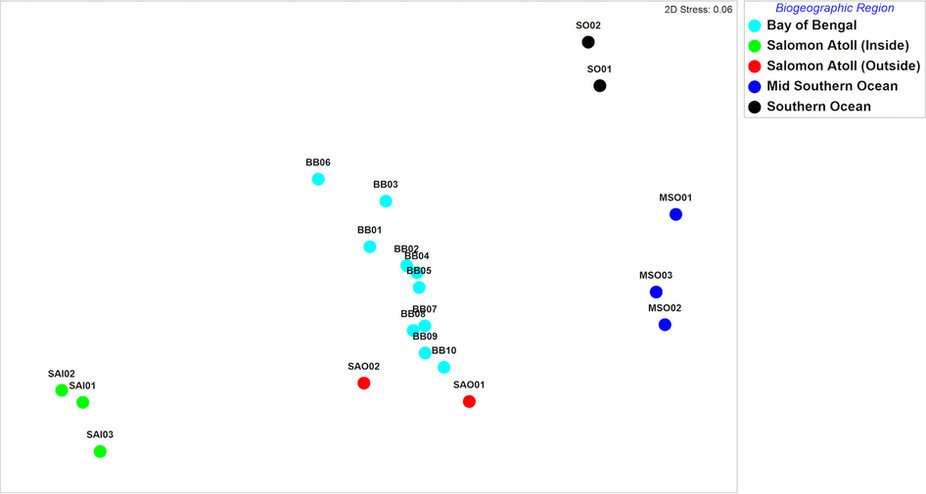
\includegraphics[width=\textwidth]{Chagos/figures/fig2}
    \caption{\textbf{MultiDimensional Scaling (MDS) of Bray-Curtis similarity between OTU profiles from distinct water masses.} Bay of Bengal = BB, Salomon Atoll (inside) = SAI, Salomon Atoll (outside) = SAO, Mid-Latitude Southern Ocean = MSO, Southern Ocean = SO. ANOSIM Global $R = 0.93$.}
    \label{Chagos_fig2}
\end{figure}

Our observations of microbial provincialism are consistent with an increasing body of literature defining the discrete distributions of microbial communities in marine habitats \cite{brown_microbial_2009, agogue_water_2011, jeffries_substrate_2011, galand_unique_2009} individual marine microorganisms \cite{gomez-pereira_distinct_2010, brown_global_2012} and taxa incorporated into ocean current models. \cite{wilkins_advection_2013, hellweger_biogeographic_2014}

The key bacterial and archeal taxa driving the dissimilarity between water masses were identified by SIMPER analysis (Supplementary Table 1) with differences between water masses consistently driven by shifts in SAR11 clades, {\em Synechococcus}, and {\em Prochlorococcus}. Previous studies have shown that, within these taxa, different phylotypes show a strong biogeographic distribution. \cite{brown_trait_2014} For example, samples from the BB were differentiated from the adjacent MSO due to increased abundances of {\em Synechococcus} and decreased {\em Prochlorococcus}. Overall this biogeographic pattern resulted in different ratios of autotrophic cyanobacteria in each water mass with increased proportion of {\em Synechococcus} relative to {\em Prochlorococcus} in the BB and {\em Prochlorococcus} being 6-fold more abundant than {\em Synechococcus} in the MSO. There were also shifts in SAR11 ecotype abundance between these two water masses with the SAR11 surface clade 1b being more abundant in the MSO and the surface clade 1a being more abundant in the BB. The high degree of dissimilarity between the BB and the Southern Ocean (SO) was driven by increased abundances of SAR86, {\em Altermonas} and {\em Synechococcus} in the BB cluster relative to the SO and an increase in SAR11 clade 1b in the SO. These phylotype abundance patterns related to temperature and latitude are in agreement with the study of Brown et al. \cite{brown_global_2012} who reported that the ratio of the surface clades of SAR11 1b over 1a is highest in waters with temperatures 19-24\degree C. \cite{brown_global_2012} SAR86 similarly has a reduced genome, well-adapted to oligotrophic conditions and shows temperature driven patterns in abundance in marine metagenomes \cite{dupont_genomic_2012} with biogeographic patterns also reflecting substrate availability and niche competition with SAR11. \cite{dupont_genomic_2012} Marine {\em Synechococcus} populations display numerous phylogenetic clades and subclades \cite{mazard_multi-locus_2012} representing ecotypes adapted to a variety of environmental conditions such as temperature and nutritional requirements and which vary in abundance in tropical coastal and open ocean water masses. \cite{brown_trait_2014} Similarly the global distribution of {\em Prochlorococcus} populations is determined by temperature, nutrient concentrations and photosynthetically active radiation (PAR), with this cyanobacterium tending to dominante in more oligtrophic conditions \cite{brown_trait_2014} such as those found in the MSO.

Archaeal sequences were also top drivers of the biogeographic partitioning between water bodies (Supplementary Table 1) with Marine group II Archaea being more abundant in the BB samples relative to the MSO and higher in the MSO than the southernmost SO samples. Marine group I Archaea were top drivers of the dissimilarity between the SO and other water bodies due to their increased abundance in this cluster.

The eukaryote sequences identified in the amplicon dataset ranged from 4\% to 23\% of the total number of amplicons at each site. Among the most abundant eukaryotic sequences were Arthopoda (Maxillopoda) and the endosymbiotic dinoflagellates {\em Syndiniales} (Figure \ref{Chagos_fig3}a). Chloroplast sequences belonging to the algae {\em Ostreococcus} and dinoflagellate {\em Phalacroma} were also abundant.

\begin{figure}
    \centering
    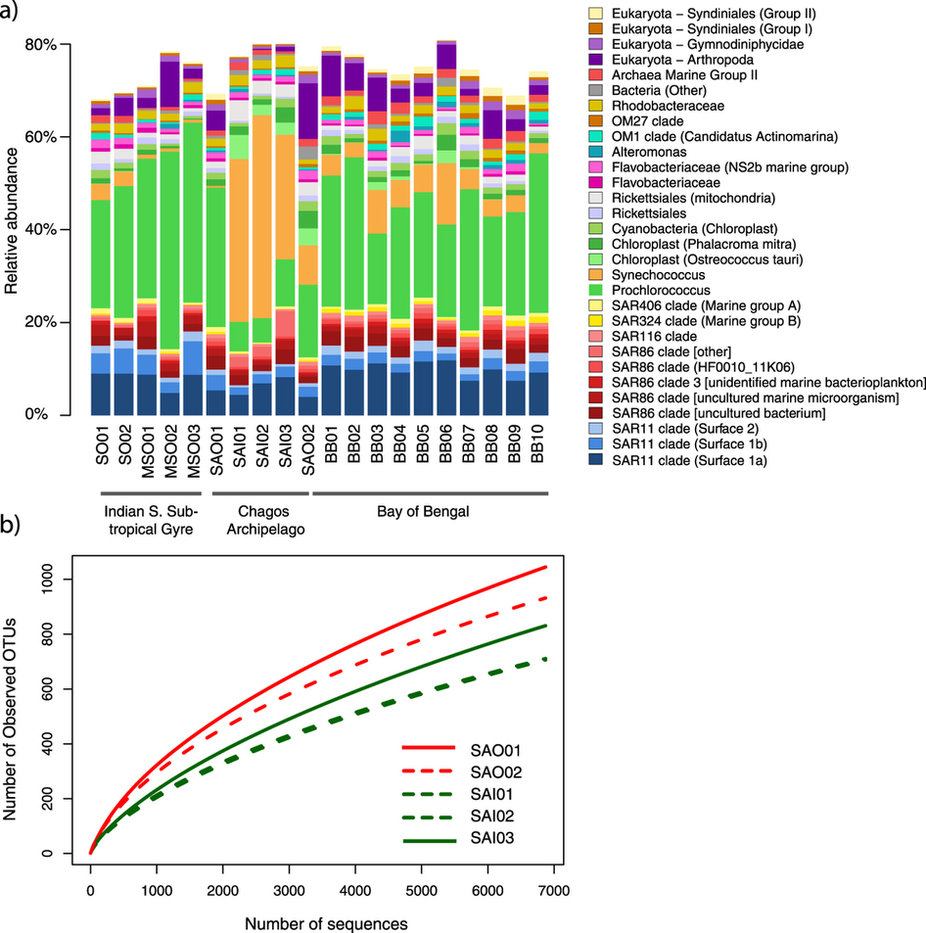
\includegraphics[width=\textwidth]{Chagos/figures/fig3}
    \caption{\textbf{Structure and richness estimates of samples from the Chagos archipelago from Illumina 16S amplicons.} \textbf{(a)} Relative abundance of most common taxa, (SILVA Database V. 119, Level 6; $>0.5\%$). \textbf{(b)} Rarefaction curves of OTU observation inside and outside of Salomon Atoll. Subsampling was performed up to the level of rarefaction (6,871 sequences per sample).}
    \label{Chagos_fig3}
\end{figure}

The abundant high-level groups (Supplementary Table 2) identified throughout the Indian Ocean include the Alveolates (Dinophyceae and Syndiniales); Metazoa (Maxillopoda); Stramenopiles (Bacilliarophyta and MAST); Hacrobia ({\em Chrysochromulina} and {\em Telonemia}) and Chlorophytes ({\em Ostreococcus}, {\em Micromonas} and {\em Bathycoccus}). Many of these eukaryotic taxa were major contributers to biogeographic patterns between water masses (Fig. 2, Supplementry Table 1). Specifically, {\em Bathycoccus} (chloroplast) was more abundant in the SO than in the BB and MSO groups and Arthropoda (Maxillopoda) was a major driver of the partitioning of BB samples away from other water masses, due to increased abundance in the northernmost parts of the transect (BB).

Overall, these specific biogeographic drivers, representing bacteria, archaea and eukarya, are abundant taxa in all samples (Figure \ref{Chagos_fig3}a). However, they are also among the most dynamic in abundance, collectively driving the top 10\% of dissimilarity. Despite this, the majority of the overall dissimilarity between water masses was driven by small contributions from taxa across all relative abundances (Supplementary Table 1) indicating that a large proportion of the community responds to the environmental variability underpinning biogeographic patterns across this $>4,000$ km transect and suggesting shifts in ecological function related to these groups.

\subsection{Biogeographic partitioning of the Salomon Islands Atoll within Chagos Archipelago}

Against the backdrop of mesoscale biogeographical patterns, the most striking demarcation is the unique structure of the microbial communities of the samples taken from within the lagoon of the Salomon Atoll. Ordination of abundance profiles (Figure \ref{Chagos_fig2}) demonstrated that samples from within the lagoon (SAI1-3) show highly discrete community composition when compared to surrounding Indian Ocean water masses. In particular, the samples did not cluster with samples located just adjacent to the lagoon (SAO1-2) despite constant water exchange and similar temperature and salinity (Table 1). These adjacent samples were more similar to Bay of Bengal samples (BB01-BB10) which clustered separately from the Southern Indian Ocean (SO01-SO02) and mid-latitude South Indian Ocean (MSO01-MSO03) samples. Similar patterns were observed using the weighted UniFrac metric (Supplementary Figure 1), with lagoon samples showing highly conserved phylogeny, which is unique to the atoll and distinct from surrounding waters. SIMPER analysis (Supplementary Table 1) indicated that the main drivers of the dissimilarity between the atoll and other samples was an increase in the cyanobacterial genus {\em Synechococcus} within the atoll, coupled to a reduction of {\em Prochlorococcus}, and shifts in the abundance of several oligotrophic SAR86 and SAR11 bacterial clades and eukaryotic sequences, in particular those belonging to the Arthropoda (Maxillopoda) (Figure \ref{Chagos_fig3}a). {\em Synechococcus} have previously been shown to play important roles in tropical lagoon systems and coral reefs playing a role in nitrogen cycling and forming the base of the food web via carbon fixation and grazing. \cite{charpy_importance_2005}

Maxillopoda (crustacea and copepod) sequences are abundant in daylit surface waters from the Southern Ocean to the Bay of Bengal (Classified as Arthropoda at level 6 of Silva119). However, they are almost absent from the daytime samples in the lagoon but increase slightly at night. (Supplementary Table 2). The Dinophyceae are represented in all samples and clustered into at least 7 major OTUs including {\em Gymnodinium fusiforme}, which is preferentially found in ocean waters outside of the Salomon Islands lagoon. Syndiniales are the most diverse high-level group with 48 OTUs and 5 major groups, including Dino-Group-II-Clade-5 and Dino-Group-I clades that are present throughout the transect but show higher abundance in the low latitude samples.

The Chlorophytes {\em Micromonas} and {\em Ostreococcus} are detected within the lagoon during the day, with decreased abundance at night, and absent or present in low abundance in the ocean samples. {\em Chrysochromulina} (Hacrobia) is another phytoplankton species that shows higher abundance within the lagoon.

\subsection{Metatranscriptional profiling of the communities from Chagos Archipelago}

We performed a survey of community level gene expression in samples from within and outside the Salomon Islands lagoon (Figure \ref{Chagos_fig4}). Unsurprisingly, among the most actively transcribed gene categories were those related to photosynthesis (Photosystem I and II), peptidoglycan, protein and fatty acid biosynthesis. A differential abundance of phycobilisome antenna transcripts was observed and attributed to the higher abundance of {\em Synechococcus} within the lagoon. In contrast there was higher {\em pcbA} gene expression outside the lagoon, which can be attributed to the chlorophyll-binding light harvesting antenna of {\em Prochlorococcus}, which represented a much larger proportion of the phototrophic community outside of the lagoon (Figure \ref{Chagos_fig3}a). Similarly, a higher abundance of retinol metabolism genes attributed to SAR86 were enriched outside of the lagoon in concordance with a higher abundance of this clade. \cite{dupont_genomic_2012} Retinol is a precursor for assembling proteorhodopsin in photo-heterotrophic bacteria \cite{delong_light-driven_2010} including SAR11 and SAR86.

\begin{figure}
    \centering
    
\includegraphics[width=\textwidth]{Chagos/figures/fig4}
    \caption{\textbf{Metatranscriptional profiling of the community outside and inside the Salomon Atoll.} \textbf{(a)} Scatter plot of log-fold change versus mean levels of transcript abundance between inside and outside water samples. The red points represents transcripts enriched or depleted in the community transcriptome under the statistical model used and the triangles are points that are outside the defined limits, in this case having a log fold value of $\pm 5.5$. The dashed lines indicate the log-fold cutoff of $\pm 1.6$. \textbf{(b)} Cartoon depicting the major differences in transcript abundance between the outside (SAO1-2), inside day (SAI1-2) and inside night (SAI3) samples.}
    \label{Chagos_fig4}
\end{figure}

Interestingly, the increased abundance in {\em Synechococcus} within the lagoon resulted in a corresponding enrichment in transcripts for exploitation of a wider range of nitrogen compounds. On average, more than 50\% of the transcripts relating to nitrogen metabolism (K00284, K00366, K00367, K01455, K01501, K01673, K01725, K01915, K02575, K15576, K15578) could be taxonomically assigned to {\em Synechococcus} compared to less than 25\% outside. Sequences of membrane transporters for urea, cyanate, nitrite/nitrate and peptides were enriched in the community transcriptome alongside genes in assimilation pathways for urea, cyanate, nitrate and glutamine, glutamate and glutathione metabolism. Outside the lagoon ammonia transport ({\em amt}) genes and broad specificity amino acid uptake ABC transporters comprised the majority of transcripts for nitrogen uptake genes. However, genes for spermidine and glycine-betaine transport systems were also more abundant in oceanic waters outside the lagoon. Spermidine has been shown to regulate the transcription of genes involved in carbon and nitrogen metabolism \cite{mou_genes_2010} and spermidine transport genes have been found in high abundance in cultured marine bacterial genomes. These observations suggest that spermidine may play an important role in regulating the nitrogen and carbon budgets of bacterioplankton. Spermidine binding proteins are also abundant in SAR11 metaproteomes from oligotrophic waters. \cite{sowell_transport_2009} Glycine-betaine is additionally a nitrogenous osmoprotectant \cite{oren_microbial_2008} that has been suggested to play a role in nutrient cycling. \cite{jeffries_increases_2012} Overall these results suggest that the shift in community composition results in a higher proportion of trascripts for nitrogen assimilation in the community inside the lagoon.

Genes involved in phosphorus uptake also showed differential patterns of transcript abundance with enrichment of organic phosphatases in oceanic waters adjacent to the lagoon and a potential phosphonate transport system enriched inside. Within the lagoon there is evidence of increased cycling of internal P into and out of polyphosphate stores with higher transcript abundance of polyphosphate kinase ({\em ppk}) and polyphosphatase genes. A recent study by Zhang {\em et al}. \cite{zhang_phosphorus_2015} reported elevated concentrations of polyphosphate granules in the tissues of reef sponges. The polyphosphate was shown to come from cyanobacterial symbionts and suggested to have important implications in the recycling of phosphate in the reef ecosystem. The taxonomic assignment of the majority of the ppk transcripts to Synechococcus (91\% inside the lagoon vs. 7\% outside) suggests this might be a possible mechanism providing planktonic cyanobacteria in the lagoon ability to grow on polyphosphate as the sole source of P. \cite{mazard2012dissecting}

The high proportion (up to 61\%) of phototrophic sequences in transcript and SSU rRNA datasets suggests that conditions within the lagoon support enhanced primary productivity (Supplementary Figure 2). Recruitment of mRNA sequences to available genome sequences show the lagoon is inhabited by cyanobacterial populations closely related to {\em Synechococcus} sp. WH8109, a representative of marine Clade II(a) (average nucleotide identity +97\% across 95.5\% of the genome; Supplementary Figure 3). {\em Synechococcus} Clade II(a) is widespread across (sub)tropical oceanic waters \cite{mazard2012dissecting, huang_novel_2012} but has been observed as a dominant phototroph in the nutrient rich waters of the Mauritanian upwelling. \cite{zwirglmaier_basin-scale_2007}

Against a backdrop of strong diel variation in {\em Synechococcus} transcript abundance, overall patterns in similarity between metatranscriptomes (Supplementary Figure 4) showed that the night sample from inside the lagoon was more similar to day samples from outside the lagoon. This suggested that the activity of {\em Synechococcus} during the day was a major driver of transcriptional differences between communities inside and outside the lagoon that was not observed at night, which is supported by the observation that genes involved in photosynthesis were among the main drivers determining this ordination (Supplementary Table 3). Interestingly, this pattern was not observed using RiboTagger abundance of transcribed SSU rRNA genes (Supplementary Figure 5), showing the same patterns as SSU rDNA OTU profiles, in which daytime and nighttime profiles were highly similar and clustered away from those outside of the lagoon. This indicated that the demarcation between night and day metatranscriptomes from the lagoon was not merely a reflection of the taxonomic composition of active microbes, but was a genome wide transcriptional response.

Samples within the lagoon were characterised by lower diversity than those adjacent (Figure \ref{Chagos_fig3}b), with a lower richness of OTUs occurring within the lagoon. This phenomenon might be analogous to the small island effect \cite{macarthur1967theory} that suggests that species richness decreases with the decrease in habitat diversity below a certain threshold in island size. However, this would imply the existence of physical barriers to dispersal, which are unlikely due to the extensive mixing of water between the lagoon and the outside ocean. Analogous strong biogeographic patterns have been previously observed for Pacific coral atolls and attributed to `bottom-up' forcing factors such as steep gradients in nutrient availability within lagoon waters. \cite{charpy_picophytoplankton_1999}

\subsection{Viral ecological filtering underlines the biogeographical singularity of the Salomon Islands.}

As an alternative or complementary top down explanation of reduced diversity and discrete biogeography within the lagoon, we report an increase in the expression of viral-related genes inside the lagoon (Figure \ref{Chagos_fig5}). Using the KEGG Orthology (KO) database, we observed within the lagoon more than 5-fold enrichment in transcripts associated with increased phage activity such as {\em pspA} (which encode phage shock protein A, K03969) and phage DNA polymerase (K02334) (Figure \ref{Chagos_fig5}a). In addition, a search of the mRNA against the database of Phage Orthologous Groups (POG) \cite{kristensen_orthologous_2013} showed that transcripts encoding T3/T7-like RNA polymerase (POG0019), terminase large sub-unit (POG0252) and a structural protein (POG1117) were also significantly higher inside the lagoon (Figure \ref{Chagos_fig5}b; Supplementary Table 4). This suggests that phages might provide the ecological filter that drives the shift in cyanobacterial populations. \cite{bowler_genetics_2014, kao_diel_2005}

\begin{figure}
    \centering
    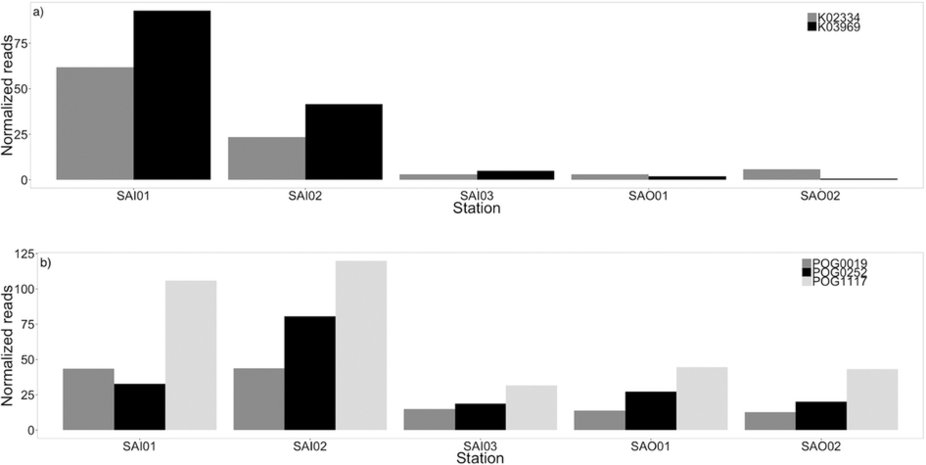
\includegraphics[width=\textwidth]{Chagos/figures/fig5}
    \caption{\textbf{Transcript abundance of viral genes inside and outside the Salomon Island Atoll.} \textbf{(a)} KEGG Orthology (KO): Grey bar represents the number of mRNA reads associated with DNA polymerase B bacteriophage-type (K02334) while the black bar represent the number of mRNA reads associated with phage shock protein A (K03969, {\em pspA}) for the station inside and outside the island atoll. The numbers of reads were normalised to 1 million reads using the total amount of reads. \textbf{(b)} Phage Orthologous groups (POGs): The dark grey bar represents the number of mRNA reads associated with T3/T7-like RNA polymerase (POG0019), the black bar represents the number of mRNA reads associated with terminase large sub-unit (POG0252) and the light grey bar represents the number of mRNA reads associated with a structural gene (POG1117) for the station inside and outside the island atoll. The numbers of reads were normalised to 1 million reads using the total amount of reads.}
    \label{Chagos_fig5}
\end{figure}

Multiple lines of evidence support this hypothesis. First the observed increase in phage activity was only evident in the daytime samples, suggesting that it is linked to active primary production (Figure \ref{Chagos_fig5}), as cyanophage production is believed to also show a diel pattern. \cite{kao_diel_2005}

Second the identity of phage transcripts within the lagoon argues for the induction of prophages from within cyanobacterial genomes. Indeed, most of the hits for the phage DNA polymerase were similar to a phage SPO1 DNA polymerase-related protein that is found in sequenced {\em Synechococcus} genomes. It is likely that the steep transition from the oligotrophic open ocean to the highly productive environment of the lagoon would be hostile to pelagic populations of {\em Prochlorococcus} and {\em Synechococcus} and the exposure to higher amounts of UV light or the change in host abundance \cite{paul_prophages_2008} would trigger prophage induction. This is reflected in the more than 4-fold enrichment in POG1405 (high-light inducible protein) transcripts observed in the diurnal samples of the lagoon (Supplementary Table 4).

These observations underline that, unlike coastal waters \cite{wilcox_bacterial-viruses_1994, weinbauer_lysogeny_1999} where phage production is primarily due to lytic infection, rather than induction of lysogenic bacteria, the increase of viral-related genes expression might be the reponse of the induction of lysogenic pelagic cyanobacteria.

Third, the lower diversity observed within the lagoon waters (Figure \ref{Chagos_fig3}b) supports the notion of periodic clonal sweeps \cite{rodriguez-brito_application_2006} with numerical dominance during the daytime by the most fit ecotypes, while at night the diversity increases (Fig. 3b) as new immigrant populations enter the lagoon through tidal and wind-driven mixing. In fact, the mRNA recruitments of the dominant {\em Synechococcus} genotypes showed pronounced shifts between day and night samples (Figure \ref{Chagos_fig6}) with immigrant populations, recruiting to clades I, VIII and sub clusters 5.2 and 5.3 genomes, being reduced during the daytime. The nocturnal immigration and diurnal selection of oceanic communities is also corroborated by amplicon data showing higher relative abundance in the night sample (SAI03) of heterotrophic taxa characteristic of waters from outside the lagoon (e.g. SAR11 and SAR86; Figure \ref{Chagos_fig3}a).

\begin{figure}
    \centering
    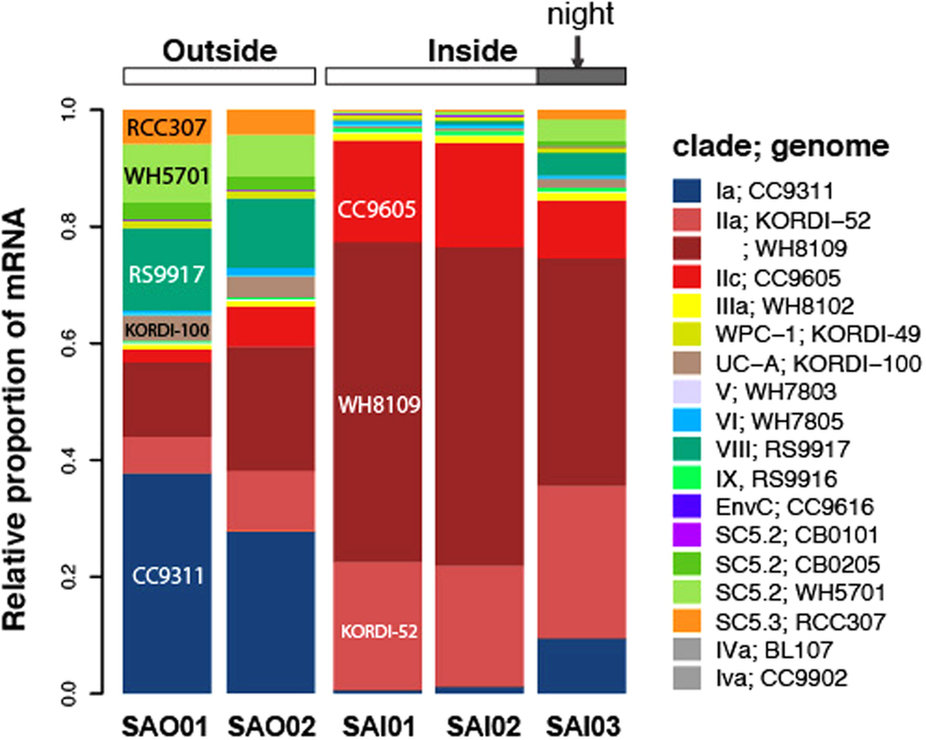
\includegraphics[width=\textwidth]{Chagos/figures/fig6}
    \caption{\textbf{Relative abundance of {\em Synechococcus} genotypes inferred from genome recruitment of transcripts comparing inside and outside Salomon Islands.}}
    \label{Chagos_fig6}
\end{figure}

The precise nature of the forces maintaining the species-area relationships within the waters of the Salomon Islands is beyond the scope of this study, but given the role of diversity in maintaining the resilience of an ecosystem, \cite{elmqvist_response_2003} we posit that the microbial assemblages within the atoll are potentially more vulnerable to perturbations and anthropogenic impact than the surrounding oceanic ecosystem.

Strong patterns were observed in taxonomic composition across oceanic provinces and within the Salomon Islands. Gaining a deeper understanding of the function of these communities is essential to predict the ecological role of microorganisms in the system and measure their response to environmental change.
